\documentclass{article}
\usepackage{latexsym}
\usepackage{amssymb,amsmath}
\usepackage{custom2}
\usepackage{graphicx} % for figures
\usepackage{epstopdf} % so can use EPS or PDF figures
\usepackage{caption}
\usepackage{subcaption}
\usepackage{url}
\usepackage{amssymb,amsfonts}
\usepackage[all,arc]{xy}
\usepackage{enumerate}
\usepackage{mathrsfs}
\usepackage{booktabs}
\usepackage[pdftex]{hyperref}
\usepackage{lscape}
\usepackage{xcolor}
\usepackage{natbib}

\captionsetup{justification=RaggedRight, singlelinecheck=false}
\newcommand{\ra}[1]{\renewcommand{\arraystretch}{#1}}
\newcommand{\argmax}{\text{argmax}}
\newcommand{\Tr}{\text{Tr}}
%\newtheorem{claim}{Claim}
\newtheorem{ass}{Assumption}

\addtolength{\evensidemargin}{-.5in}
\addtolength{\oddsidemargin}{-.5in}
\addtolength{\textwidth}{1.4in}
\addtolength{\textheight}{1.4in}
\addtolength{\topmargin}{-.5in}

\pagestyle{empty}

\begin{document}
\begin{center}
\Large

\end{center}


\vspace{0pt}

\begin{center}
{\bf \LARGE{Stochastic Learning Dynamics with Two Applications}}
\end{center}

\tableofcontents

\section{Abstract}
Learning usually occurs in noisy environments.  In order to make a decision, one must accumulate the  evidence for different alternatives and choose one only once the uncertainty about the choice is sufficiently reduced.  There are two biological systems in which the variables used to make a decision can be described by a random walk: the firing rates of neural populations in the brain of an individual making a decision about a visual stimulus and the beliefs of monkeys about their relative dominance based on the fights they have engaged in.  The same stochastic differential equations can be used to model these quite different systems, which suggests that there are universal principles underlying learning through noisy dynamical systems.  In the neural system, the differential equations are often reduced to a one-dimensional model, but the social system is inherently two-dimensional.  The thresholds dictating when a decision has been made affect both the accuracy of the decision and the expected time until a decision is reached. We find that the dimensionality of the decision process does not affect its accuracy.  We find that if a pair of individuals optimize their thresholds to avoid waiting, a pair making an easy decision will take more time than a pair making a difficult decision.  In a group of individuals optimizing their thresholds to avoid waiting, those pairs making the difficult decisions about high value inputs will have to wait the longest.  Finally, the skewness of the power distribution in the social system is maximized at intermediate waiting costs and the information content of the power distribution is higher when the individual maximize their probability of becoming dominant rather than the accuracy of their decisions. In comparing the output of the model of the social system to data, we found that ...

\section{Introduction}

\subsection{Neural }
Stochastic differential equations have been used to model, explain, and predict learning and decision making in both monkeys and humans \citep{Eckhoff:2008uq, Brown:2005fk,Feng:2009kl,Bogacz:2006uq}.  Typically, an experimental subject is presented with a visual stimulus that consists of dots, some percentage of which are moving coherently either left or right and the rest of which are moving randomly.  The subject is then asked to decide in which direction the dots were moving.  If there are two neural populations, each of which fire in response to a particular direction of motion, the firing rates of the two populations will tend to increase or decrease, depending on the strength and direction of the stimulus.  Eventually, either the experimenter forces a decision to be made, in which case whichever population has a higher firing rate determines which decision is made, or the firing rate of one population becomes high enough that the subject decides for that direction.  To summarize, there are two decision variables--- the firing rates of two neural populations responding to left and right motion--- that perform a biased random walk until enough evidence has been accumulated to make a decision one way or the other.


\subsection{Social }
In groups of pigtailed macaques, different animals have different fighting abilities, and when a pair of animals engages in a fight, one animal may be more likely on average to ``win" the fight.  Over time, as one animal learns that it is likely to lose fights, it will decide to emit a formal subordination signal, communicating its agreeing to the subordinate role in their relationship \citep{Flack:2007kx, Flack:2006fk,Flack:2004oq, Waal:1985fk,Caldecott:1986uk}.  The outcome of a fight is affected by each animal's allies, the presence of those allies, motivation levels,  external environmental variables, and other factors.  Additionally, the number of fights that occur in any period of time depends on similarly stochastic factors.  Because of this stochasticity, the number of fights won and lost in any period of time is a random variable.  Each animal's opinion about its relative dominance, therefore, will perform a biased random walk until one animal's opinion of itself is low enough to agree to being subordinate.

Similar models have previously been applied to animal conflicts, although in that case the model assumed that the animals had perfect memory of their past interactions \citep{Froment:2010fk}

\subsection{Extent and Limits of Analogy }

In Table \ref{variables}, we list the inputs, decision variables, and outputs of the two systems.  

%In the neural system, an individual wants to make both a decision that is both quick and accurate.  This is also true in the social system.  However, it may also be the case that a monkey wants to avoid emitting a subordination signal and wants to receive a signal, regardless of whether or not this is the ``correct" outcome, i.e. whether or not he is actually more likely to win a fight.  The criterion used to optimize the threshold, therefore, may be quite different in the two systems.  Additionally, the speed and outcome of the decision process depend on both individuals' thresholds.  Since an individuals' best behavior depends on the behavior of the other animal, optimizing the threshold has a strategic aspect.  


\section{The model \label{derivation}}
\subsection{Stochastic differential equations }
Learning systems have been successfully modeled with stochastic differential equations \citep{Eckhoff:2008uq, Brown:2005fk,Feng:2009kl,Bogacz:2006uq}, although the application of this type of model has been quite phenomenological.  With two assumptions about the timescales on which probabilistic events occur, a simple mechanistic description of the accumulation of information about random events can be turned into a stochastic differential equation \cite{Gillespie:2000fk}.  

%note about applicability to quorum sensing?!?

In the absence of any input, the decision variables leak back towards $0$ with rate $\ell$.  (A table of all variables used in the text is given in Table \ref{variables}.)  If there is no input, then over a period of time of length $\tau$ a decision variable would decrease as $X(t+\tau)=(1-\ell\tau)X(t)$.  There are two types of inputs: in the neural system, a dot can move either left or right and in the social system a fight can be won by one animal or another.  For clarity in the following we will refer to these left or right dots, but the biological interpretation of the two types of inputs depends on the system.  Each decision variable responds positively to one type of input and negatively to the other, with the signs of their responds the opposite of each other.  Specifically, in the neural case, one neural population responds positively to left dots and negatively to right dots and the other neural population does the opposite.  In the social case, one animal's estimate of its own dominance increases when it wins fights and decreases when it loses fights, and the other animal's estimate does the opposite.  

To determine the estimate at time $t+\tau$, we can count how many times each of type of input occurred in the time since $t$ and add the changes resulting from these events to the background leaky estimate (as in \cite{Gillespie:2000fk}):
\begin{align*}
X_1(t+\tau)&=(1-\ell\tau)X_1(t)+b\times\# \text{ of left dots in }[t,t+\tau)-b\times\# \text{ of right dots in }[t,t+\tau)
\\ X_2(t+\tau)&=(1-\ell\tau)X_2(t)-b\times\# \text{ of left dots in }[t,t+\tau)+b\times\# \text{ of right dots in }[t,t+\tau). 
\end{align*}
where $b$ is the change caused by a single input.

Our first assumption is that the rates at which the two types of inputs occur is constant.  We can thus describe the number of each type of event with a Poisson random variable, $N_\text{L}$ and $N_\text{R}$.  We rewrite our basic equations to give 
\begin{align*}
X_1(t+\tau)&=(1-\ell\tau)X_1(t)+bN_\text{L}-bN_\text{R}
\\ X_1(t+\tau)&=(1-\ell\tau)X_2(t)-bN_\text{L}+bN_\text{R}.
\end{align*}
If events happen at a rate $r$ and the event is a left dot with probability $c$ and a right dot with probability $1-c$, then the expectation of $N_L$ and $N_R$ in a period of length $\tau$ are, respectively, $\tau r c$ and $\tau r(1-c)$. In the neural case, $c$ is related to the ``coherence'' of the visual stimulus.  A $c$ close to $0$ or $1$ means that most of the events are of one type or the other and the decision is easier to make than when $c$ is close to $.5$.

If enough events happen in the period of time from $t$ to $t+\tau$ then we can approximate the Poisson random variables with Normal random variables with mean and variance equal to the mean of the Poisson random variables.  Our second assumption, then, is that the period of time of length $\tau$ is long enough to make this approximation. Let $Z_\text{L}$ and $Z_\text{R}$, be independent standard Normal random variables, i.e. with mean $0$ and standard deviation $1$.  Then our equations for $X_i(t+\tau)$ become
\begin{align*}
X_1(t+\tau)&=(1-\ell\tau)X_1(t)+b\bigg(\tau rc+\sqrt{\tau rc}Z_{\text{L}}\bigg)-b\bigg(\tau r(1-c)+\sqrt{\tau r(1-c)}Z_{\text{R}}\bigg)
\\X_2(t+\tau)&=(1-\ell\tau)X_2(t)-b\bigg(\tau rc+\sqrt{\tau rc}Z_{\text{L}}\bigg)+b\bigg(\tau r(1-c)+\sqrt{\tau r(1-c)}Z_{\text{R}}\bigg).
\end{align*}
Finally, as we make the period of time shorter and shorter, making $\tau$ infinitesimally small, these equations become stochastic differential equations,
\begin{equation}
\begin{array}{ll}
dX_1&=\bigg(-\ell X_1(t)+br(2c-1)\bigg)dt+\bigg(b\sqrt{rc}\bigg)dW_\text{L}t-\bigg(b\sqrt{r(1-c)}\bigg)dW_\text{R}t
\\dX_2&=\bigg(-\ell X_2(t)-br(2c-1)\bigg)dt-\bigg(b\sqrt{rc}\bigg)dW_\text{L}t+\bigg(b\sqrt{r(1-c)}\bigg)dW_\text{R}t
\end{array}
\end{equation}
where $dW_{\text{L}}$ and $dW_{\text{R}}$ are independent Brownian motions representing, respectively, the left and right inputs.  The assumptions about the timescales on which inputs occur are particularly reasonable in the social system, although the successful application of this type of model to neural populations implies they are not unreasonable in that system.

%\begin{equation}
%\begin{array}{ll}
%dX_1&=\bigg(-\ell X_1(t)+b(2d-1)\bigg)dt+b\sqrt{d}dW_{1}t-b\sqrt{(1-d)}dW_{2}t
%\\dX_2&=\bigg(-\ell X_1(t)+b(1-2d)\bigg)dt-b\sqrt{d}dW_{1}t+b\sqrt{(1-d)}dW_{2}t,
%\end{array}
%\end{equation}
\subsection{Reaching a decision }
Each decision variable, $X_1$ and $X_2$, accumulates information about the stimulus.  The sign and size of the two variables indicate how much evidence there is for each possible decision outcome.  When a lot of evidence for the first possibility has been observed, $X_1$ will be large and positive, and similarly for the second possibility.  If the difference in the variables can be observed, the difference indicates the relative strengths of the evidence for either possibility. If $Y=X_1-X_2$, when $Y$ is large enough the system decides on $X_1$ and when $Y$ is low enough the system decides on $X_2$.  Specifically, there are two thresholds, $T_2$ and $T_1$ such that if $Y>T_1$ the decision is for $X_1$ and if $Y<-T_2$ the decision is for $X_2$.  However, it may be the case that the difference in the variables cannot be observed.  In this case, the decision depends on whether $X_1$ or $X_2$ hits a threshold first.  Again, there are two thresholds, $T_2$ and $T_1$, and if $X_1<-T_1$ the decision is for $X_1$ and if the $X_2<-T_2$ the decision is for $X_2$. 

In the neural system, the two stochastic equations describing the activity of the two neural populations integrating environmental evidence are often reduced to the one-dimensional equation describing the difference in the activity levels to make the system easier to analyze \cite{Brown:2005fk,Bogacz:2006uq,Feng:2009kl}.  However, in the social system we are considering, we cannot make any assumptions about the existence of a third party evaluating the difference in the opinions of the two animals.  A ``decision," i.e. the emission of a signal from one of the two animals, is only reached when one of the two animals' opinions goes below a certain threshold.  The social system is therefore inherently two-dimensional, whereas the neural system may be adequately described by one dimension.   

\subsection{Utility of the decision }
The thresholds affect the expected time until a decision is reached (decision time, DT) and the probability that an incorrect decision is made (error rate, ER).  The thresholds also affect the probability that either variable will ``give up'' first.  In the social case, this is the probability that each animal will emit a subordination signal (signaling probability, $\text{SP}_i$).  In the neural case, ??? These quantities, DT, ER, and $\text{SP}_i$, satisfy partial differential equations with respect to the starting values of the decision variables. In Appendix \ref{pdes_deriv}, we derive these partial differential equations.  While an analytical solution is known in the one-dimensional case, the two-dimensional case is analytically intractable.  We therefore numerically solve the PDEs in the two-dimensional case.  In Table \ref{models}, we compare how the decision is made and how the decision process is optimized in the two systems.

The quality of the decision process depends on each of these three quantities.  The lower the decision time and error rate, the better the decision.  However, both cannot be decreased simultaneously so there is a tradeoff that depends on how the two quantities are prioritized.  Additionally, in the social case, each animal may benefit from lower its signaling probability, which may or may not conflict with lowering the error rate, depending on whether the animal is weaker or stronger than its opponent.  To quantify the utility of the decision process, we introduce three weights, $w_1$, $w_2$, and $w_3$, which determine how the three quantities are prioritized.  For animal $i$, we define
\begin{equation*}
U_{i}=w_1\text{DT}+w_2\text{ER}+w_3\text{SP}_i.
\end{equation*}
The decision is better if $U_i$ is lower.  In the social system, $w_2$ can be interpreted as the cost of fighting since when $w_2$ is higher, the time spent fighting until a decision is reached is more costly.  Similarly, $w_3$ can be interpreted as the benefit from being the dominant animal in a pair.


%A drift diffusion model is equivalent to a sequential probability ratio test, a learning algorithm that is optimal with respect to its accuracy and the time required to make a decision \cite{Moehlis:2004fk,Bogacz:2006uq}.  

\subsection{Optimal thresholds }
An individual-- either a neural population or a monkey-- can be engaged in either a single decision or in many decisions at once.  In the social system, for example, an animal wants to decide whether it is dominant or subordinate to every other member of its social group.  For any pair of individuals, each has a utility, $U_1$ and $U_2$, and consequently each has a Nash equilibrium threshold such that, if they choose those thresholds, neither has an incentive to choose another.  Similarly, in a group of individuals, each animal $i$ has a utility $U_{ij}$ from its decision process with animal $j$.  These lead to an optimized set of thresholds such that no individual has an incentive to choose another threshold.

Since an individual is trying to use the same algorithm to learn about every other animal, he is constrained to have only one decision threshold for each of these decision processes.  The optimal decision threshold in this group context depends on the distribution of difficulties ($c$) of the decision an individual will have to make and the thresholds of the other individuals.  In the social system, the distribution of difficulties ($c$) comes from the distribution of fighting abilities of the animals.  

 We use the following procedure to find optimal thresholds as a function of position in the group.  We repeatedly draw a set of fighting abilities from a uniform distribution; we find the optimal thresholds for each set, and then find the average optimal threshold as a function of an animal's order in the set of fighting abilities. To find the optimal thresholds for a given set of fighting abilities, we turn the difference in fighting abilities between each pair into the difficulty of the decision they have to make ($c$).  For an initial set of thresholds, we find $U_{ij}$ for each animal $i$ in each of its decisions and then average $\langle U_{ij}\rangle_j$ across all the animals with which it is engaged in a decision process.  We then allow each animal to choose a threshold that optimizes $\langle U_{ij}\rangle_j$ with respect to the rest of the group's thresholds and we iterate these choices until no animal chooses a new threshold.  

\subsection{Consensus }
Consensus about the value of each individual in a group emerges out of the decision process.  In the social system, an animal's social power depends on the consensus in the group about its fighting ability \cite{Flack:2004oq,Flack:2006uq,Brush:2013fk}.  Given the decisions that each pair of individuals reaches, there are measures of the consensus in the group that successfully predict an animal's social power and also extend to other social systems \cite{Brush:2013fk}.  For each random set of fighting abilities, we let the animals optimize their thresholds, which give the probability that each pair will reach either decision, and we then generate a set of decisions given by these probabilities.  These decisions then give a distribution of power among the group.  For many random sets of fighting abilities, we can find the mutual information between the power distribution and the true fighting abilities, which we call the information content of the power distribution. It tells us how informative observing the outcomes of the decisions is about the underlying fighting abilities.  We also find the average skewness of the power distributions.

\section{Results}

\subsection{Decisions are as accurate without an arbiter. }
We compare the decision making process in the full two-dimensional system and in a reduced one-dimensional system to see whether decisions are made more accurately or quickly in one or the other.  To make the systems directly comparable, we assume in both cases that the thresholds are symmetric, i.e. $T_1=T_2$.  We find that the two-dimensional decision is as accurate as the one-dimensional decision.  That is, for a given expected time to reach a decision, the two-dimensional decision will reach the correct decision with the same probability.  Accuracy decreases as leak rates ($\ell$) become higher, but increases when the strength of the input ($c$) is higher (Figure \ref{2dacc}).

Without any prior knowledge of the probabilities of the state of the external stimulus, it is reasonable to assume that the thresholds for deciding for each direction are symmetric.  On the other hand, the thresholds are chosen by two competing individuals-- neural populations or animals-- and it is possible that the two individuals have different thresholds.  The accuracy in a given amount of time depends on the ratio of the two thresholds and is improved when the weaker animal's threshold is lower than the stronger animal's threshold (Figure \ref{2dflex}).  

\subsection{Increasing waiting costs make easy decisions take longer. }

If waiting is not costly and the error rate does not matter ($w_1=0$, $w_2=0$, $w_3=1$), there is no incentive for the individuals to stop accumulating evidence (fighting, in the social case) so the Nash equilibrium thresholds are high and both individuals wait until the other gives up.  However, as waiting costs increase, the pair can reach a decision more quickly if the weaker individual lowers its threshold.  If waiting costs are high enough, the stronger individual will also lower its threshold to avoid a long decision time (Figure \ref{nasheq_thresholds}).  Pairs making difficult decisions make more accurate decisions when the costs of waiting are higher since the weaker animal has an incentive to give up more quickly (Figure \ref{nasheq_thresholds}).  For low waiting costs, pairs of individuals making a difficult decision (low $c$, e.g. animals with similar fighting abilities) will take longer to reach a decision than pairs making a difficult decision (high $c$, e.g. animals with disparate fighting abilities).  At intermediate costs, pairs of individuals making intermediate decisions will take the longest to reach a decision.  When costs are high, the pairs that take the longest to reach a decision are those making the easiest decisions (Figure \ref{nasheq_thresholds}).  

As with the Nash equilibrium thresholds, if waiting is not costly and the error rate does not matter ($w_1=0$, $w_2=0$, $w_3=1$), there is no incentive for the individuals to stop accumulating evidence (fighting, in the social case) so they will all set high thresholds.  As waiting costs increase, first weaker animals will start to lower their thresholds and then strong animals will as well (Figure \ref{groupeq_thresholds}).  For low waiting costs, pairs of animals with similar fighting abilities, and thus making difficult decisions, take the longest to reach a decision.  For high waiting costs, pairs of animals with similar and high fighting abilities take much longer, and those animals with similar and low fighting abilities will reach a decision more quickly.

\subsection{Costs affect the shape and the information content of the power distribution.  }

The average skewness of the power distribution is maximized at intermediate waiting costs ($w_2$) (Figure \ref{power}). Changing $w_1$ and $w_3$ have less of an effect, although when $w_1$ is higher the skewness slightly increases. The information content decreases as waiting costs increase.  Counterintuitively, if the individuals maximize the probability of being dominant in each of its pairs rather than the accuracy of those decisions, the information content of the power distribution increases (Figure \ref{power}).  In other words, the information in all of the group's decisions is higher when the accuracy of pairwise decisions decreases.

\subsection{Comparison to social data }
Empirically, those pairs of monkeys that take the longest to establish a signaling dynamics are those with the most similar fighting abilities...

\section{Discussion}

\begin{figure}[ht]
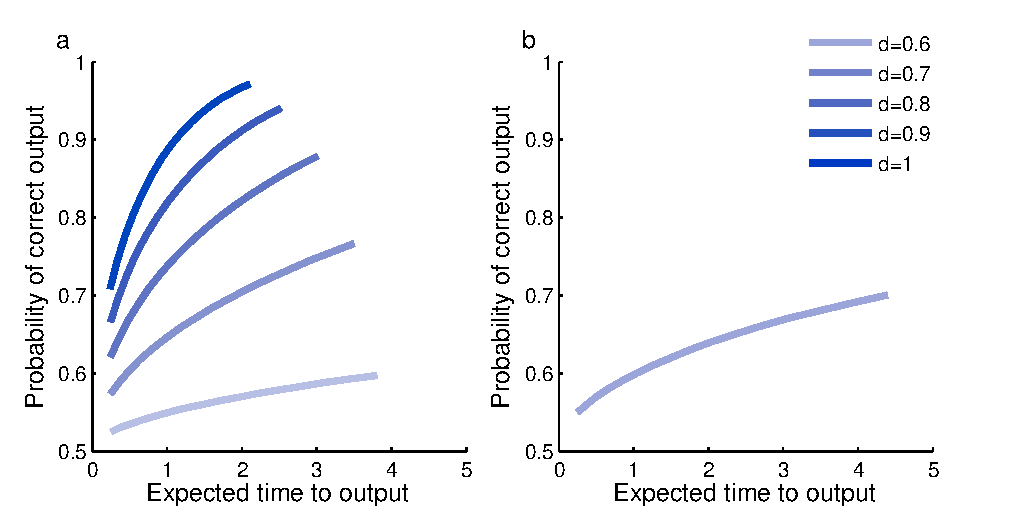
\includegraphics[width=\textwidth]{2d_accuracy.pdf}
\caption{\label{2dacc} }
\end{figure}

\begin{figure}[ht]
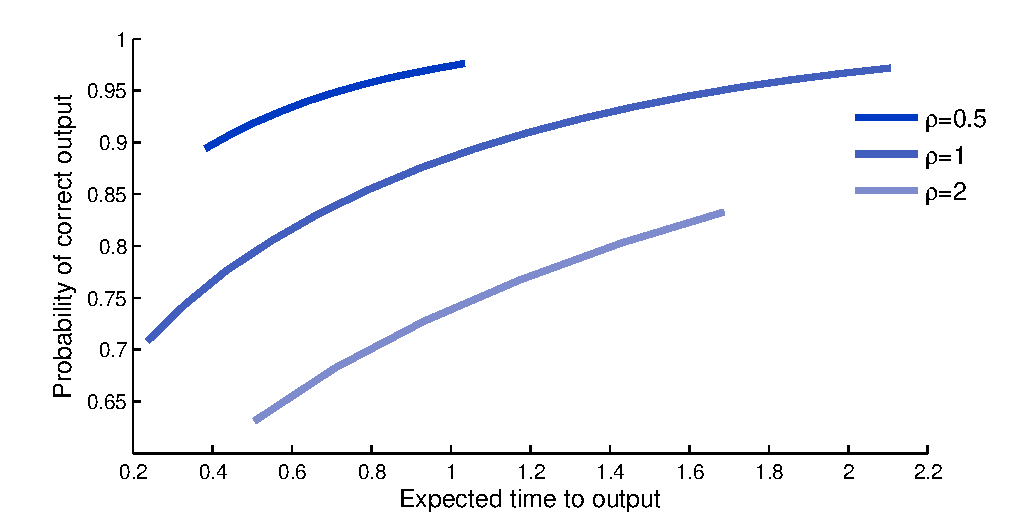
\includegraphics[width=\textwidth]{2d_flexible_thresholds.pdf}
\caption{\label{2dflex} When the two thresholds in the two-dimensional system are allowed to vary freely, the decision process can be arbitrarily accurate in a given amount of time, depending on how much lower the weaker animal's threshold is than the stronger animal's threshold.  The expected time to reach a decision is on the x-axis and the probability of reaching the correct decision in that amount of time is on the y-axis.  The curve depends on the ratio of the weaker animal's threshold to the stronger animal's threshold ($\rho$).  Lower ratios are represented in higher darker curves.}
\end{figure}

\begin{figure}[ht]
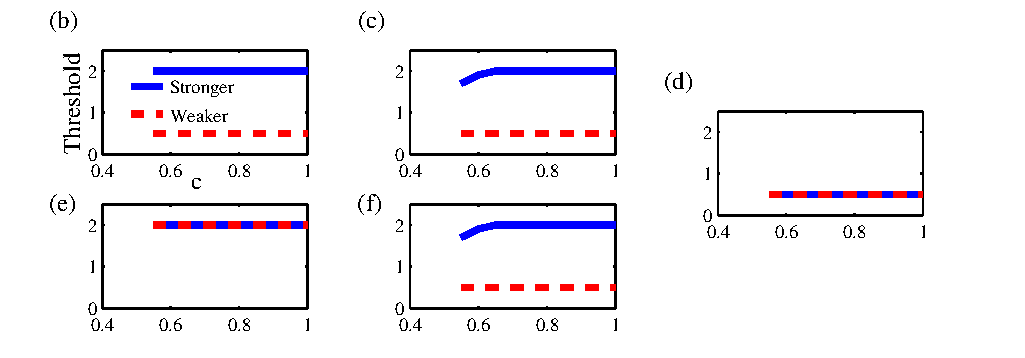
\includegraphics[width=\textwidth]{nasheq_thresholds.pdf}
\caption{\label{nasheq_thresholds} If a pair of individuals optimize their thresholds in response to each other, as the costs of waiting increase, first the weaker individual will start to lower his threshold to avoid waiting for a long time and then the stronger individual will start to lower his threshold as well.  As the costs of waiting increase, first the accuracy with which a pair can make a difficult decision increases and then it decreases.  At low waiting costs, difficult decisions take the most time.  At intermediate costs, intermediate decisions take the most time.  At high costs, easy decisions take the most time. The first row of panels shows the Nash equilibrium thresholds as a function of the difficulty of the decision ($c$ close to $.5$ is a more difficult decision).  The second and third rows show, respectively, the probability of the pair reaching the correct decision and the expected time until a decision is reached, if the pair of individuals uses the Nash equilibrium thresholds.  Each column corresponds to a particular waiting cost and the cost increases from left to right ($w_1=0, w_3=1-w_2$).  }
\end{figure}

\begin{figure}[ht]
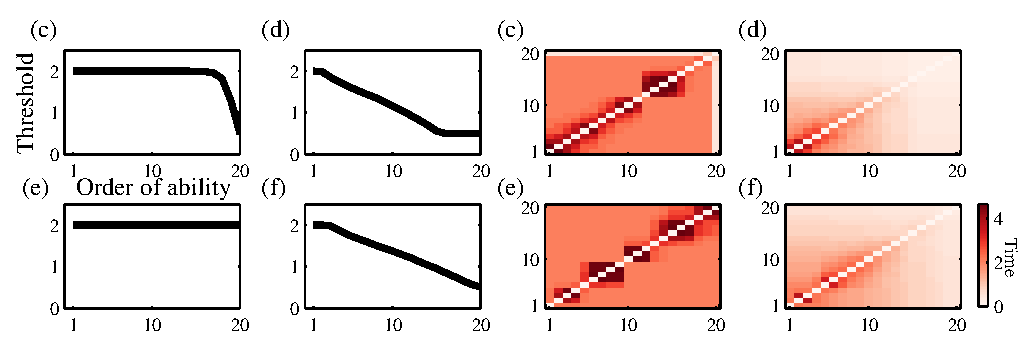
\includegraphics[width=\textwidth]{groupeq_thresholds.pdf}
\caption{\label{groupeq_thresholds} If the animals optimize their thresholds with respect to the thresholds and fighting abilities of the whole group of animals, as the costs of fighting increase, first the weaker animals in the group lower their thresholds to avoid fighting for a long time with the stronger animals and then the stronger animals lower their thresholds as well.  The ability of to learn from an animal's signaling behavior decreases as the costs of fighting increase. When fighting is not costly, the pairs of animals that take longest to decide on a relationship are those with similar fighting abilities. As costs increase pairs of animals with similarly low fighting abilities resolve their relationships quickly, whereas pairs of animals with similarly high fighting abilities take a long time to resolve their relationships.  The first row of panels shows the optimal threshold as a function of the animal's true rank with respect to fighting ability.  The second row shows the mutual information between the probability of emitting a signal and the probability of being the weaker animal, as a function of the animal's true rank.  The third row shows the expected time until each pair of animals resolves their relationship.  Each column corresponds to a particular waiting cost and the cost increases from left to right ($w_1=0, w_3=1-w_2$).   }
\end{figure}

\begin{figure}[ht]
\begin{subfigure}{3.415in}
\caption{}
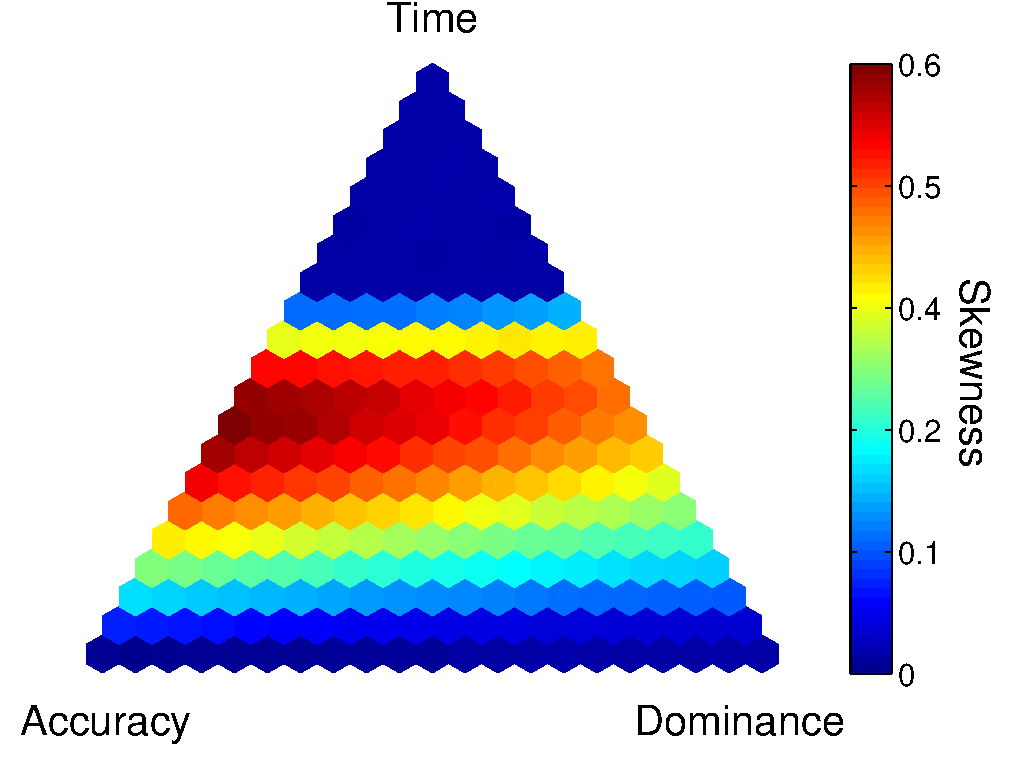
\includegraphics[width=\textwidth]{skewness_heatmap_poster.pdf}
\end{subfigure}
\begin{subfigure}{3.415in}
\caption{}
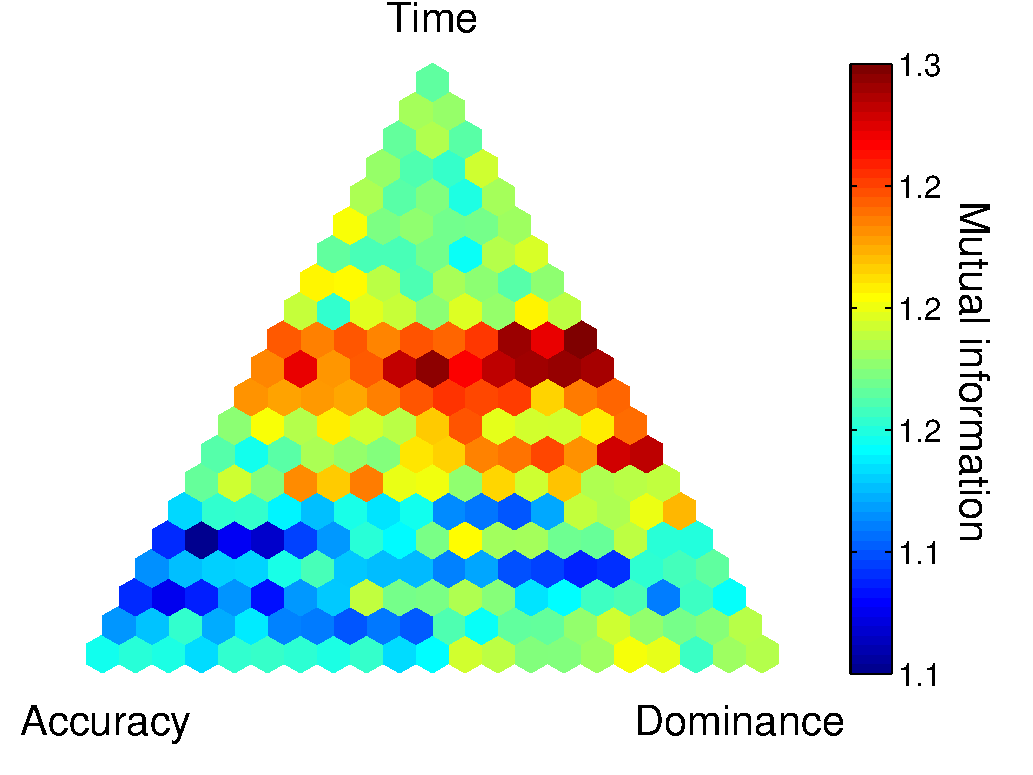
\includegraphics[width=\textwidth]{mutinfo_heatmap_poster.pdf}
\end{subfigure}
\caption{\label{power} Average skewness of the power distribution is maximized at intermediate waiting costs. The information content of the power distribution always increases as waiting costs decrease and when the benefits of being dominant increase.  The simplex shows the possible combinations of priorities, $w_1$, $w_2$, and $w_3$ such that the three weights sum to $1$.  In the lower left corner, $w_1=1$ (only accuracy matters), in the upper corner $w_2=1$ (only waiting time matters), and in the lower right $w_3=1$ (only the probability of receiving the signal matters).  The heatmaps show (a) the skewness of the power distribution and (b) the mutual information of the power distribution when the animals in the group optimize their thresholds according to those weights.  
%Increasing or decreasing $c_2$ has the strongest effect.  Increasing $c_1$ slightly increases the skewness. 
}
\end{figure}

\begin{table}[ht]
\centering
\caption{\label{variables}{\bf  Variables and interpretations in neural and social systems.} }
\ra{1.3}
\begin{tabular}{@{}rllll@{}}
Variable & Interpretation & Neural &   Social \\
\cmidrule{1-4} 
& input & dots moving left or right & fights won or lost
\\$c$ & strength of input & coherence of dots & probability of stronger animal winning
\\$X_1,X_2$ & decision variables &  firing rates of neural populations & opinions about relative dominance
\\ & dist. of states of the world & left / right equally likely & distribution of fighting abilities
\\ & decision & subject indicates left or right & one animal emits a subordination signal
\\ & correct decision & subject chooses correct direction & weaker animal signals
\end{tabular}
\end{table}

\begin{table}[ht]
\centering
\caption{\label{models}{\bf  Comparison of models applied to neural and social systems.} Differences are highlighted in red.}
\ra{1.3}
\begin{tabular}{@{}rllll@{}}
& \multicolumn{2}{c}{Neural} &  Social \\
\cmidrule{2-3} \cmidrule{4-4} 
%model  & DDM or OU & race && race with leak
%\\
dimensionality & $1$  && $2$
\\decision & difference hits a threshold  && \fcolorbox{red}{white}{one var. hits a threshold}
\\ optimality criterion &  reward from being ``right" && reward from being ``right"
\\ & reward rate && reward rate
\\ & Bayes risk && Bayes risk
\\ & && \fcolorbox{red}{white}{reward from  receiving signal}
\\optimization depends on & input strength && input strength
\\ & noise && noise
\\ & leak rate && leak rate
\\ & && \fcolorbox{red}{white}{other animal's threshold}
\\threshold  algorithm & error correction
\\  & hill climbing
\end{tabular}
\end{table}

\pagebreak
\section{Appendix}

\subsection{Derivation of PDEs for waiting time and accuracy \label{pdes_deriv}}

\pagebreak
\nocite{*}
\bibliographystyle{plain}
\bibliography{signaling_model}

\end{document}


